\documentclass[11pt]{amsart}
\usepackage{geometry}                % See geometry.pdf to learn the layout options. There are lots.
\geometry{letterpaper}                   % ... or a4paper or a5paper or ... 
%\geometry{landscape}                % Activate for for rotated page geometry
%\usepackage[parfill]{parskip}    % Activate to begin paragraphs with an empty line rather than an indent
\usepackage{graphicx}
\usepackage{amssymb}
\usepackage{epstopdf}
\usepackage[usenames,dvipsnames]{color}
\usepackage{hyperref}
\hypersetup{colorlinks=true}
\DeclareGraphicsRule{.tif}{png}{.png}{`convert #1 `dirname #1`/`basename #1 .tif`.png}
\renewcommand\familydefault{\sfdefault}
\newcommand{\todo}[1]{{\bf\textcolor{red}{TODO: #1}}}
\setlength{\topmargin}{0cm}
\setlength{\headheight}{0cm}
\setlength{\headsep}{1cm}
\setlength{\textheight}{7.7in}
\setlength{\textwidth}{6.5in}
\setlength{\oddsidemargin}{0cm}
\setlength{\evensidemargin}{0cm}
\setlength{\parindent}{0.25cm}
\setlength{\parskip}{0.1cm}

\usepackage{fancyhdr,graphicx,lastpage}% http://ctan.org/pkg/{fancyhdr,graphicx,lastpage}
\fancypagestyle{plain}{
  \fancyhf{}% Clear header/footer
  \fancyhead[L]{CSCI-GA.3033-018 - Geometric Modeling}% Right header
  \fancyhead[R]{
\includegraphics[height=20pt]{nyu.pdf}}% Right header
  \fancyfoot[L]{\vspace{2pt} Daniele Panozzo}% Left footer
  \fancyfoot[R]{\vspace{2pt} \thepage}% Right footer
}

\pagestyle{plain}% Set page style to plain.
\begin{document}

\hspace{50pt}

\begin{center}

{\Huge \textbf{Assignment 1: Hello World}}\\
\vspace{10pt}
\end{center}

In this exercise you will
\begin{itemize}
\item{Familiarize yourself with \texttt{libigl} and the provided mesh viewer.}
\item{Get acquainted with some basic mesh programming by evaluating surface
    normals, computing mesh connectivity and isolating connected components.}
\item{Implement a simple mesh subdivision scheme.}
\end{itemize}

\section{First steps with \texttt{libigl}}
The first task is to familiarize yourself with some of the basic code
infrastructure provided by \texttt{libigl}. 

\subsection{Eigen}
\texttt{libigl} uses the \href{http://eigen.tuxfamily.org/}{\texttt{Eigen}}
library for all of its matrix computations. In \texttt{libigl}, a mesh is typically
represented by a set of two \texttt{Eigen} arrays, V and F. V is a float or
double array (dimension \#V $\times$ 3 where \#V is the number of vertices) that
contains the positions of the vertices of the mesh, where the i-th row of V
contains the coordinates of the i-th vertex. F is an integer array (dimension
\#faces $\times$ 3 where \#F is the number of faces) which contains the
descriptions of the triangles in the mesh. The i-th row of F contains the
indices of the vertices in V that form the i-th face, ordered counter-clockwise. 

Check out the
\href{http://eigen.tuxfamily.org/dox/GettingStarted.html}{"Getting Started"}
page of \texttt{Eigen} as well as the
\href{http://eigen.tuxfamily.org/dox/group__QuickRefPage.html}{Quick Reference}
page to acquaint yourselves with the basic matrix operations supported.

Note that you need not install Eigen manually since a reasonably up-to-date
version is included as a submodule in \texttt{libigl}.

\subsection{Installing \texttt{libigl} and Running the Tutorials}
If you haven't already, install \texttt{libigl} by following the
instructions in the ``General Rules and Instructions'' handout.
Next, build the tutorials: \\
\texttt{cd \$LIBIGL\_ROOT/; mkdir build; cd build; cmake ..; make -j2}.\\
This can take a while, so be sure to set the "-j" flag to run on as many cores
as possible.

\noindent Each tutorial is named with format \texttt{XXX\_TUTORIAL\_NAME},
where \texttt{XXX} is the number ID of the tutorial. After the build completes,
each tutorial executable can be run, e.g.: \texttt{./XXX\_TUTORIAL\_NAME\_bin} 

\noindent The source code for the corresponding tutorial is located in \\
 \texttt{\$LIBIGL\_ROOT/tutorial/XXX\_TUTORIAL\_NAME/main.cpp}

\noindent Experiment with the basic functionality of \texttt{libigl} and the
        included mesh viewer by running at least the first 6 tutorials and
        inspecting the corresponding source code. 

\section{Neighborhood Computations}
For this task, you will use \texttt{libigl} to perform basic neighborhood
computations on a mesh. Computing the neighbors of a mesh face or vertex is
required for most mesh processing operations, as you will see later in the
class. For this task, you need to fill in the appropriate sections (inside the
keyboard callback, keys '1' to '2') of \texttt{src/main.cpp} to compute the
neighborhood relations using \texttt{libigl}. In order to use a
function from \texttt{libigl} (e.g. the function to compute per-face normals),
you must include the relevant header file at the top of your \texttt{main.cpp}
file (e.g. \texttt{\#include <igl/per\_face\_normals.h>}) and call it later in
your code (\texttt{igl::per\_face\_normals(V,F,FN)}).

\subsection{Vertex-to-Face Relations}
Given V and F, generate an adjacency list which contains, for each vertex, a
list of faces adjacent to it. The ordering of the faces incident on a vertex
does not matter. Your program should print out the vertex-to-face relations in
text form when key '1' is pressed.

\emph{Relevant} \texttt{libigl} \emph{functions: } \texttt{igl::vertex\_triangle\_adjacency}.

\subsection{Vertex-to-Vertex Relations}
Given V and F, generate an adjacency list which contains, for each vertex, a
list of vertices connected with it. Two vertices are connected if there exists
an edge between them, i.e., if the two vertices appear in the same row of F. The
ordering of the vertices in each list does not matter.  Your program should
print out the vertex-to-vertex relations in text form when key '2' is pressed.

\emph{Relevant} \texttt{libigl} \emph{functions: } \texttt{igl::adjacency\_list}.

\subsection{Visualizing the Neighborhood Relations}
Check your results by comparing them to the built-in relations calculated by the
mesh viewer. You can do this by clicking on the checkboxes ``Show vertex
labels'' and ``Show faces labels'' in the viewer window.
\vspace{0.5cm}

Required output of this section:
\begin{itemize}
\item{A text dump of the content of the two data structures for the provided
    mesh ``plane.off''.}
\end{itemize}

\section{Shading}
For this task, you will experiment with the different ways of shading discrete
surfaces already implemented in \texttt{libigl}. Fill in the appropriate source
code sections (inside the keyboard callback, keys '3' to '5') to display the
mesh with the appropriate shading.

\subsection{Per-face Shading}
\begin{figure}[h!]
   \centering
   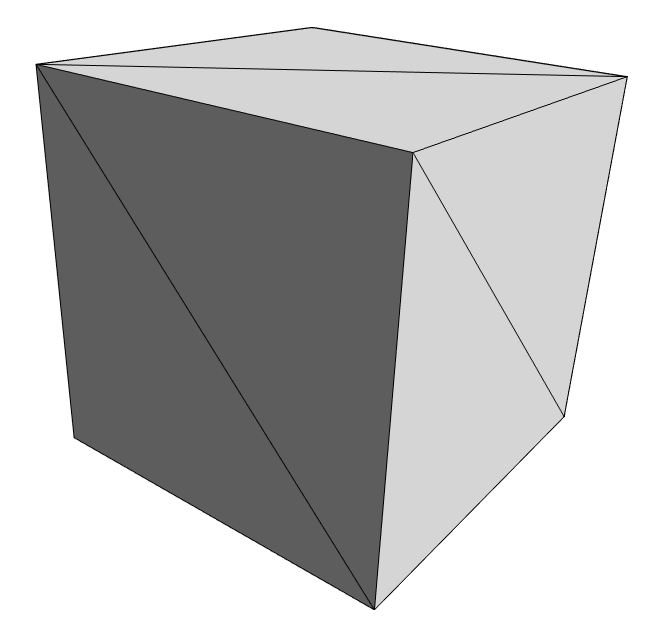
\includegraphics[scale=0.18]{cube_face.png} % requires the graphicx package
\hspace{3cm}
   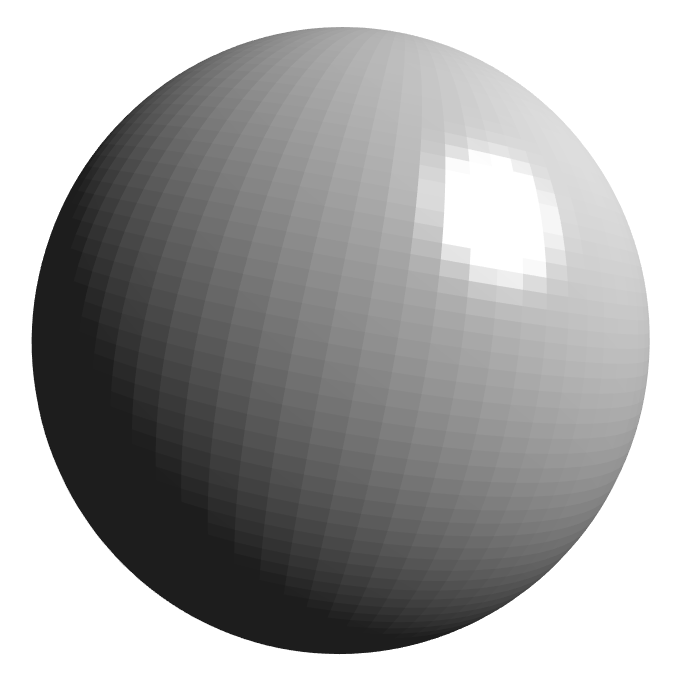
\includegraphics[scale=0.18]{sphere_face.png} % requires the graphicx package
   \caption{Flat Shading}
   \label{fig:flat_shading}
\end{figure}

The simplest shading technique is flat shading, where each polygon of an object
is colored based on the angle between the polygon's surface normal and the
direction of the light source, their respective colors, and the intensity of the
light source. With flat shading, all vertices of a polygon are colored
identically. Your program should compute the appropriate shading normals and shade
the input mesh with flat shading when the key '3' is pressed.

\emph{Relevant} \texttt{libigl} \emph{functions: }
\texttt{igl::per\_face\_normals}. Call \texttt{viewer.data.set\_normals($\cdot$)} to
set the shading in the viewer to use the normals you computed.

\subsection{Per-vertex Shading}
Flat shading may produce visual artifacts, due to the color discontinuity
between neighboring faces. Specular highlights may be rendered poorly with flat
shading. When per-vertex shading is used, per-vertex normals are computed for
each vertex by averaging the normals of the surrounding faces. Your program
should compute the appropriate shading normals and shade the input mesh with
per-vertex shading when the key '4' is pressed.

\emph{Relevant} \texttt{libigl} \emph{functions: }
\texttt{igl::per\_vertex\_normals}. Call \texttt{viewer.data.set\_normals($\cdot$)} to
set the shading in the viewer to use the normals you computed.

Compare the result must be compared with the one obtained with flat shading.
\begin{figure}[h!]
   \centering
   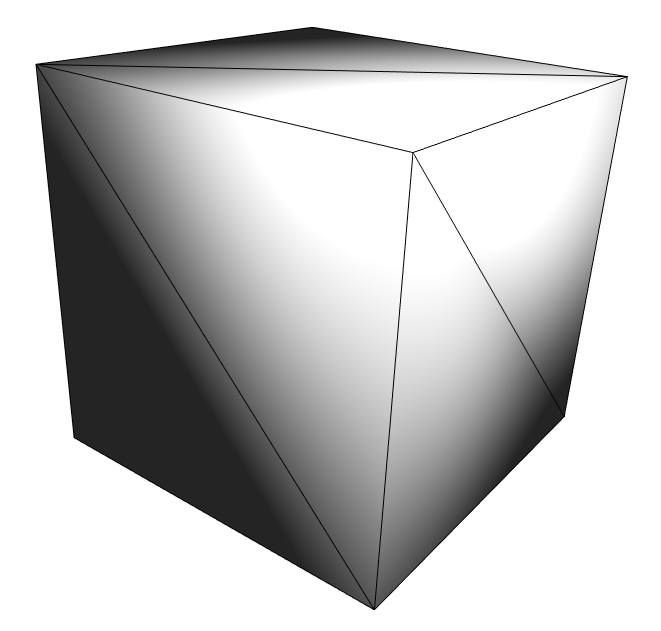
\includegraphics[scale=0.18]{cube_vertex.png} % requires the graphicx package
\hspace{3cm}
   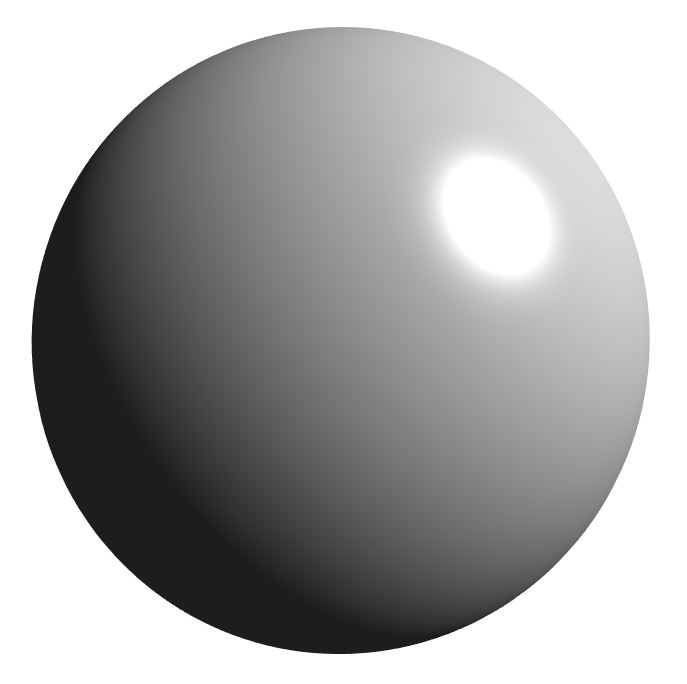
\includegraphics[scale=0.18]{sphere_vertex.png} % requires the graphicx package
   \caption{Per-Vertex Shading}
   \label{fig:per_vertex_shading}
\end{figure}

\subsection{Per-corner Shading}
On models with sharp feature lines, averaging the per-face normals on the feature, as done for per-vertex shading, may result in blurred rendering. It is possible to avoid this limitation and to render crisp sharp features by using per-corner normals. In this case, a different normal is assigned to each face corner; this implies that every vertex will get a (possibly different) normal for every adjacent face. A threshold parameter is used to decide when an edge belongs to a sharp feature. The threshold is applied to the angle between the two corner normals: if it is less than the threshold value, the normals must be averaged, otherwise they are kept untouched.  Your program should compute the appropriate shading normals (with a threshold of your choice) and shade the input mesh with per-vertex shading when the key '5' is pressed.

\emph{Relevant} \texttt{libigl} \emph{functions: }
\texttt{igl::per\_corner\_normals}. Call
\texttt{viewer.data.set\_normals($\cdot$)} to set the shading in the viewer to
use the normals you computed.

Compare the result must be compared with the one obtained with flat and per-vertex shading. Experiment with the threshold value.

\begin{figure}[h!]
   \centering
   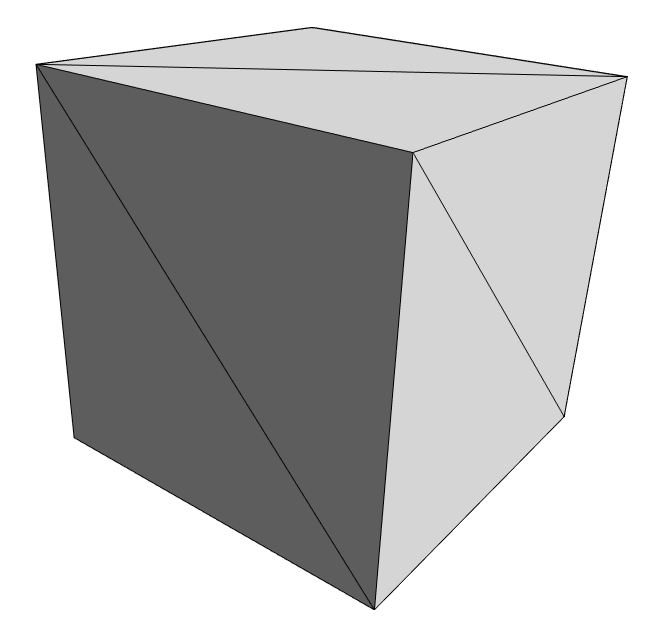
\includegraphics[scale=0.18]{cube_corner.png} % requires the graphicx package
\hspace{3cm}
   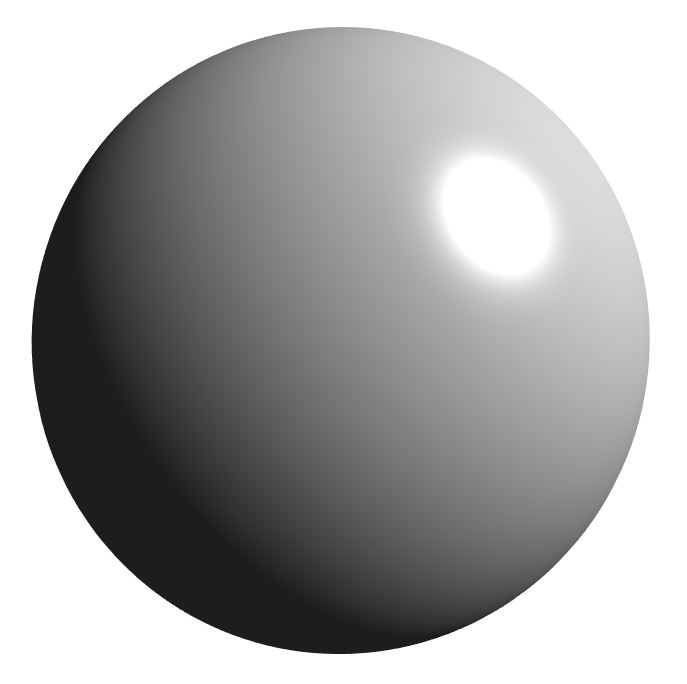
\includegraphics[scale=0.18]{sphere_corner} % requires the graphicx package
   \caption{Per-Corner Shading}
   \label{fig:per_corner_shading}
\end{figure}

\vspace{1cm}
Required output of this section:
\begin{itemize}
\item{Screenshots of the provided meshes shaded with flat, per-vertex, and per-corner normals.}
\end{itemize}


\section{Connected Components}
Using neighborhood connectivity, it is possible to partition a mesh into
connected components, where each mesh face belongs only to a single
component. Fill in the appropriate source code sections (inside the keyboard
callback, key '6') to display the mesh with each face colored to indicate the
component it belongs to (coloring each component distinctly).
You can use the jet colormap provided with \texttt{libigl} to assign colors to
the components, or you can implement your own colormap.

\emph{Relevant} \texttt{libigl} \emph{functions: }
\texttt{igl::facet\_components, igl::jet}. Call
\texttt{viewer.data.set\_colors($\cdot$)} to set the displayed colors to the
per-face colors you computed.

\begin{figure}[h!]
   \centering
   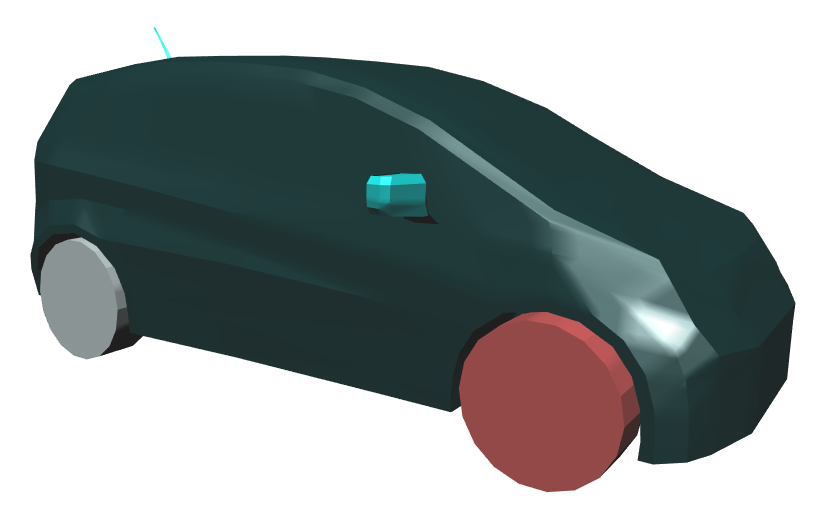
\includegraphics[width=0.6\columnwidth]{car.png} % requires the graphicx package
\hspace{3cm}
   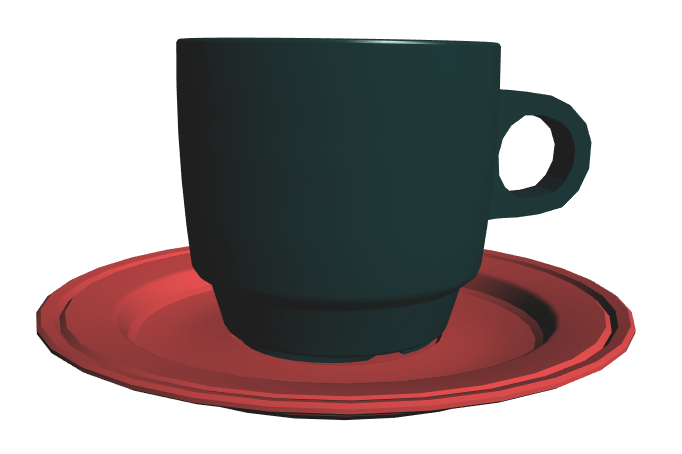
\includegraphics[width=0.5\columnwidth]{cup.png} % requires the graphicx package
   \caption{Connected components visualized by coloring each component
    distinctly.}
   \label{fig:conn_comp}
\end{figure}

\vspace{0.5cm}

Required output of this section:
\begin{itemize}
\item{Screenshots of the provided meshes with each connected component colored differently.}
\item{The number of connected components and the size of each component (measured in number of faces) for all the provided models.}

\end{itemize}


\section{A simple subdivision scheme}
\begin{figure}[h!]
   \centering
   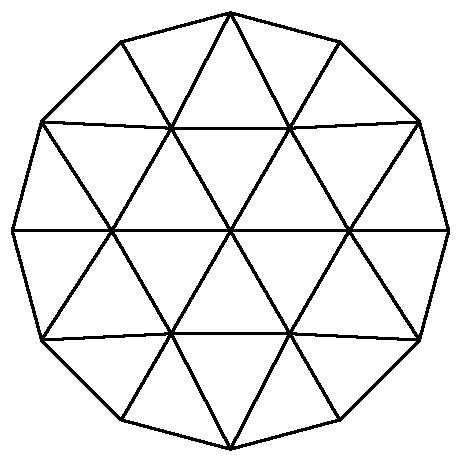
\includegraphics[width=0.24\columnwidth]{sqrt31-1.png}
%\hspace{3cm}
   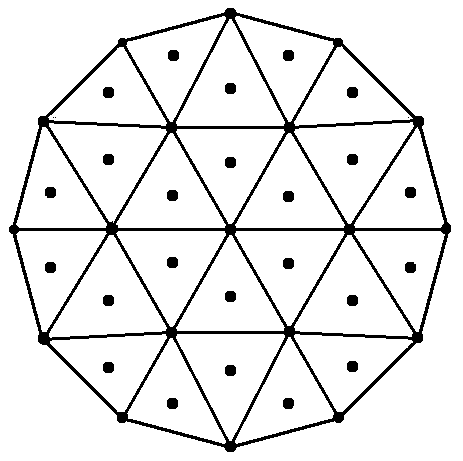
\includegraphics[width=0.24\columnwidth]{sqrt31-2.png}
%\hspace{3cm}
   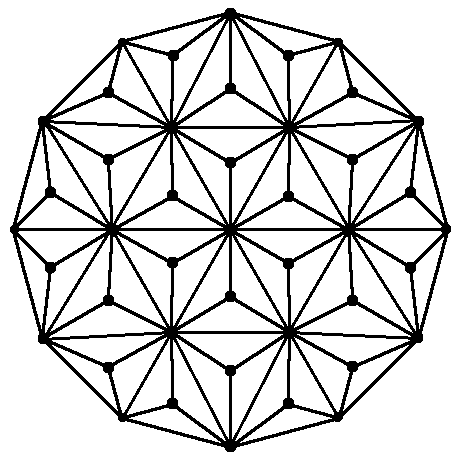
\includegraphics[width=0.24\columnwidth]{sqrt31-3.png}
%\hspace{3cm}
   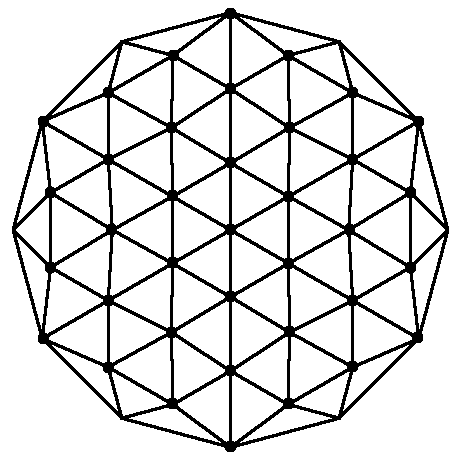
\includegraphics[width=0.24\columnwidth]{sqrt31-4.png} % requires the graphicx package
   \caption{$\sqrt{3}$ Subdivision. From left to right: original mesh, added
    vertices at the midpoints of the faces (step 1), connecting the new points
    to the original mesh (step 1), flipping the original edges to obtain a new
    set of faces (step 3). Step 2 involves shifting the original vertices and is
    not shown.}
   \label{fig:subdivision1}
\end{figure}

For this task, you will implement the subdivision scheme described in
\cite{Kobbelt00sqrt(3)-subdivision}
(\url{https://www.graphics.rwth-aachen.de/media/papers/sqrt31.pdf}) to
iteratively
create finer meshes from a given coarse mesh. According to the paper, given a
mesh (V,F), the $\sqrt{3}$-subdivision scheme creates a new mesh (V',F')
by applying the following rules:
\begin{enumerate}
\item Add a new vertex at location $\mathbf{m}_f$ for each face $f \in F$ of the
    original mesh. The new vertex will be located at the midpoint of the face.
        Append the newly created vertices $M = \{\mathbf{m}_f\}$ to V to create
        a new set of vertices $V'' = [V;M]$. Add three new faces for each face
        $f$ in order by connecting $\mathbf{m_f}$ with edges to the original 3
        vertices of the face; we call the set of this newly created faces $F''$.
        Replace the old set of faces $F$ with $F''$.
\item Move each vertex $\mathbf v$ of the old vertices V to a new position
    $\mathbf p$ by averaging $\mathbf v$ with the positions of its neighboring
        vertices in the \emph{original} mesh. If $\mathbf v$ has valence $n$ and
        its neighbors in the original mesh (V,F) are located at $\mathbf v_0,
        \mathbf v_1, \ldots, \mathbf v_n$, then the update rule is 


\begin{displaymath}
\mathbf p = (1-a_n)\mathbf v + \frac{a_n}{n}\sum\limits_{i=0}^{n-1}\mathbf v_i
\end{displaymath}

\noindent where $a_n = \frac{4-2\cos\left(\frac{2\pi}{n}\right)}{9}$. The vertex
        set of the subdivided mesh is then $V' = [P,M] $, where $P$ is the
        concatenation of the new positions $\mathbf p$ for all vertices.

\item { Replace the $F''$ with a new set of faces $F'$ such that the edges
    connecting the newly added points $M$ to $P$ (the relocated original
        vertices) remain but the original edges of the mesh connecting points in
        $M$ to each other are flipped. See
        Figure~\ref{fig:subdivision1}. }
\end{enumerate}



\begin{figure}[h!]
   \centering
   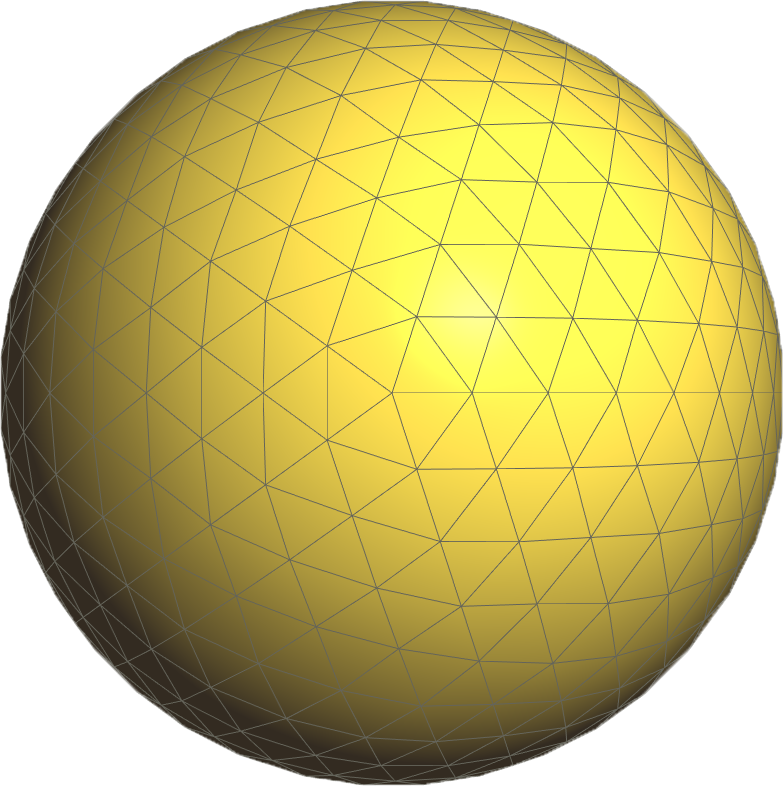
\includegraphics[width=3.8cm]{sphere_before}
%\hspace{3cm}
   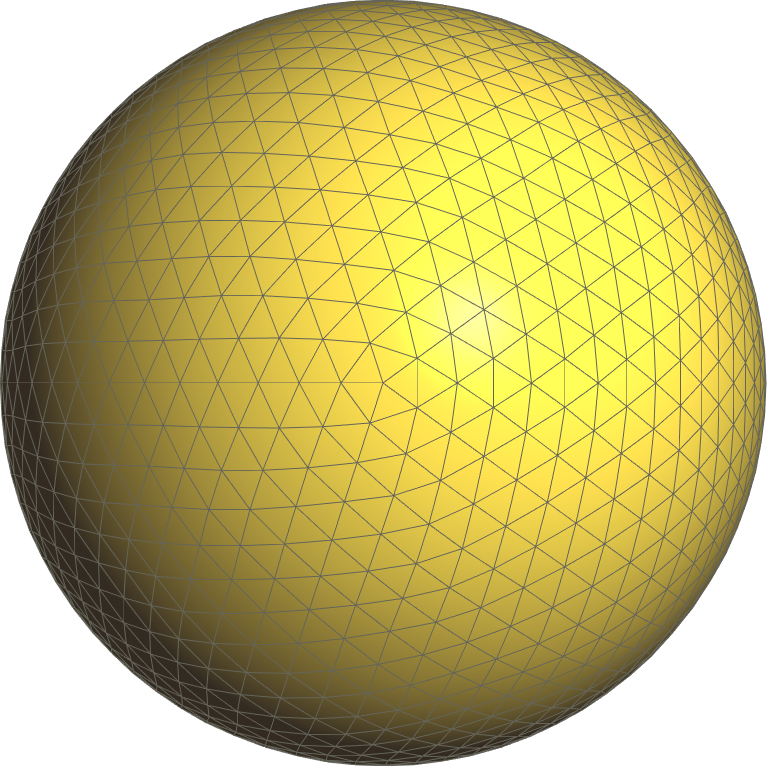
\includegraphics[width=3.8cm]{sphere_after}
\hspace{.2cm}
   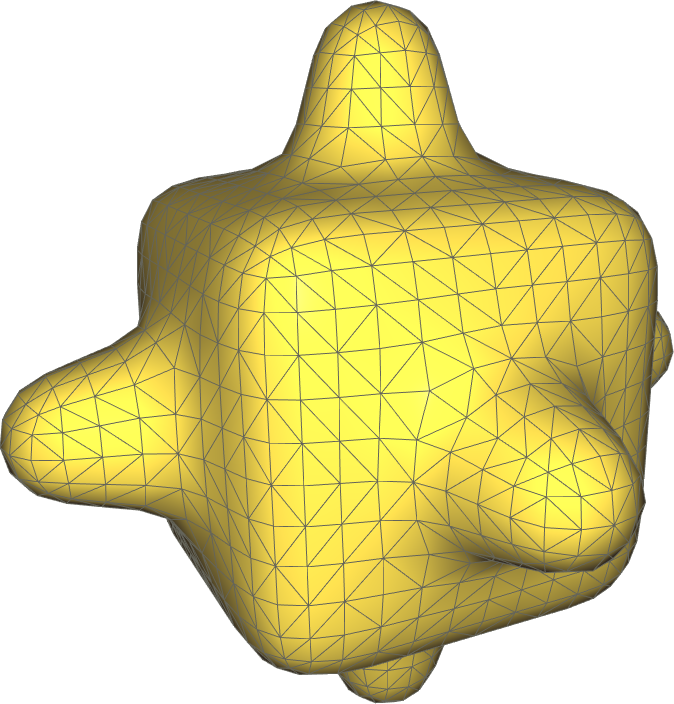
\includegraphics[width=3.8cm]{bumpy_before}
%\hspace{3cm}
   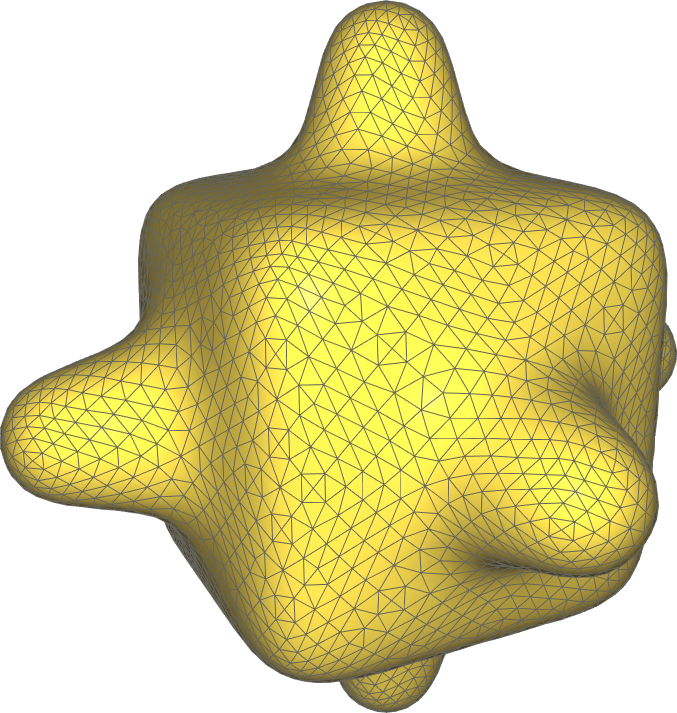
\includegraphics[width=3.8cm]{bumpy_after}
   \caption{Example of one $\sqrt{3}$ subdivision step.}
   \label{fig:subdivision2}
\end{figure}

\noindent Fill in the appropriate source code sections (inside the keyboard
callback, key '7') so that hitting key '7' subdivides the mesh once and displays
it in place of the old mesh. 

\emph{Relevant} \texttt{libigl} \emph{functions: } Many options possible. Some
suggestions: \texttt{igl::adjacency\_list},
\texttt{igl::triangle\_triangle\_adjacency}, \texttt{igl::edge\_topology},
\texttt{igl::barycenter}. Use \texttt{viewer.data.clear()} and
\texttt{viewer.data.set\_mesh($\cdot$,$\cdot$)} to replace the displayed mesh in
the viewer.

\vspace{0.5cm}

Required output of this section:
\begin{itemize}
\item{Screenshots of the subdivided meshes.}
\end{itemize}

\bibliographystyle{plain}
\bibliography{bib.bib}
\end{document}  
